\chapter{Core concepts}

%core concepts
%- myšlenka překládání - dotazy lze zrychlit použitím jiného ORM
%- idea abstrakce - složitost 2N místo N\^2
%- overview co je potřeba přeložit
%- výběr 3 frameowrků pro překlad

After analyzing several ORMs we have discovered differences between them, yet at their core their purpose remains identical. The primary objective is to retrieve data via querying using a defined set of rules for transforming database records into application objects.

Let us consider an example. In \autoref{sec:perf_eval}, specifically query \hyperref[query:d3]{D3}, we tested retrieving one-to-many optional relationship.
EF Core took more than 2.5 seconds. Compare it to the best result---linq2db scoring 91 milliseconds. That is more than a 20 times increase in speed! 

Multiple ORMs should be able to coexist in one application. When we looked at Dapper in \autoref{sec:feat_dapper}, the authors even recommended using it alongside another ORM in performance-critical areas. But converting queries between different ORMs and query languages can be a difficult process. We will focus on automating the conversion process. In addition, we will design a tool using our conversion process to compare performance of a specific query across different frameworks.

\section{Translation}

A query in a .NET application is dependent not only on the actual query statement, but also on the entity and its mapping. We have already seen how different mappings can look. The entity is always a C\# class. The mapping can vary in format and style. We have seen mapping in the form of property attributes, fluent API syntax, and even XML files. Despite the differences, the core concept remains the same. We need to tell the ORM how to map each entity to respective tables, which data types and restrictions to use, and so on. We will take a closer look at what each mapping can express and find common patterns across ORMs. 

In the same way, we will look at querying. We have seen two types - directly using raw SQL or statically typed LINQ. Actually, there was one more, lambda functions in RepoDB. But these functions can be viewed as a very limited subset of LINQ, so we will not consider them. Regardless of the query language, all queries must be translated into SQL statements when sent to the database. Therefore, SQL is actually a good base for the abstraction we can build on.

An abstraction over entities, mapping, and queries will give us a unified intermediate representation we can convert into and out of. We will only need to implement two conversions for each ORM. One to parse it into the abstract representation, and the other to build ORM-specific statements from. Instead of $N^2 - N$ conversions (one from each framework to another, except itself), only $2N$ will need to be implemented, where $N$ is the number of supported ORMs. Of course, not all directions need to be implemented. For example, translating from a deprecated ORM might be useful for migrations, but translating into it might be unnecessary.

\section{User interaction}
Input into the conversion tool will be \textbf{entity}, \textbf{mapping} and a \textbf{query}. Not all ORMs require or even support mapping, and there are different formats. So each ORM will have defined which parts it accepts. Input framework can be either auto-detected or manually selected by the user. Upon selection, multiple inputs with a description will appear.

As an example in \autoref{fig:orm_to_abstract}, the user selects Entity Framework Core as the source ORM. Given we support only attribute mapping, two inputs will be shown. One for an attributed entity and a second for a LINQ query. After user confirms 

\begin{figure}[H]
  \centering
  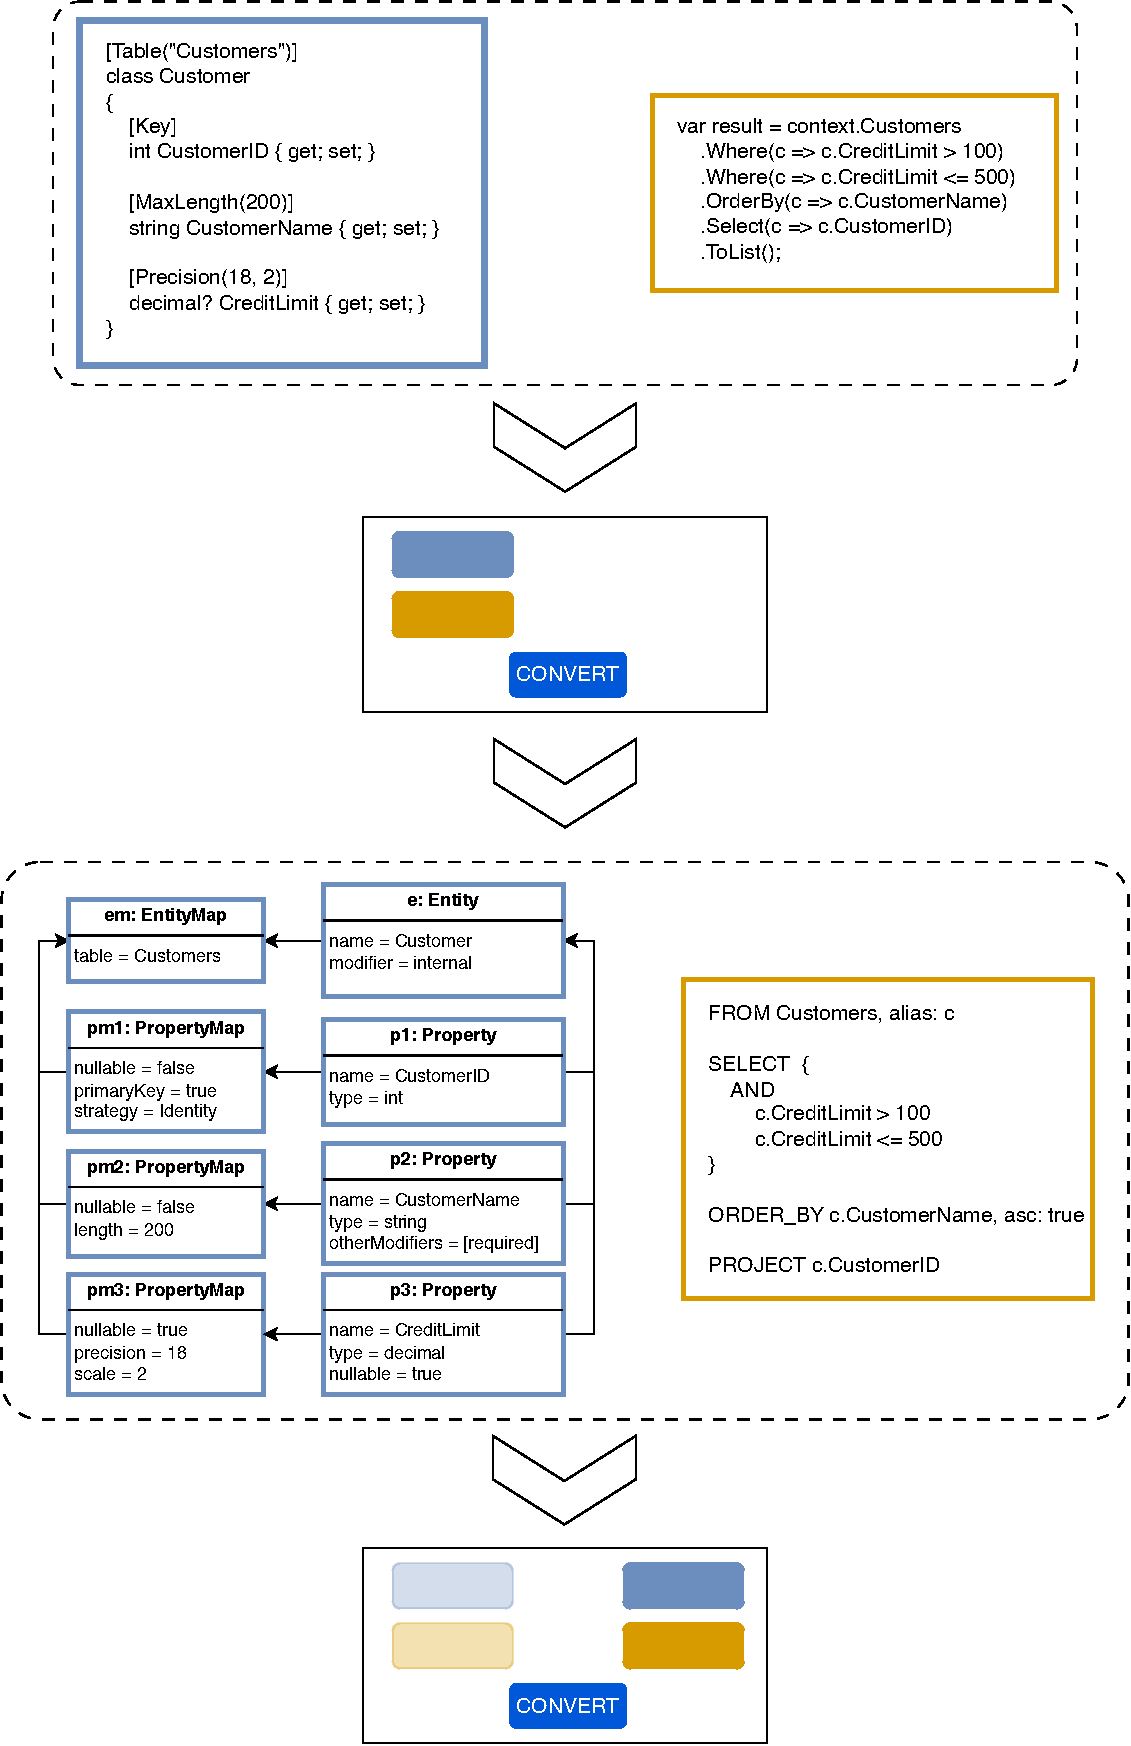
\includegraphics[width=\textwidth]{thesis/img/thesis/03_core_concepts.drawio.pdf}
  \caption{An example of entity and query being converted into abstract representation. User inputs EF Core entity and LINQ query. Our tool converts it to abstract representation, which in turn can be translated into any user selected ORM.}
  \label{fig:orm_to_abstract}
\end{figure}

\section{Advisor}
TODO advisor